\documentclass{ximera}

\newcommand{\RR}{\mathbb R}
\renewcommand{\d}{\,d}
\newcommand{\dd}[2][]{\frac{d #1}{d #2}}
\renewcommand{\l}{\ell}
\newcommand{\ddx}{\frac{d}{dx}}
\newcommand{\dfn}{\textbf}
\newcommand{\eval}[1]{\bigg[ #1 \bigg]}



\outcome{Understand linear density and its connection to mass.}
\outcome{Calculate the mass of an objection with varying density.}
\outcome{Understand work and how it is computed.}
\outcome{Calculate work when force is varying.}
\outcome{Know when to integrate a cross-section to solve a physics problem.}
\outcome{Calculate work when distance is varying.}


\title[Dig-In:]{Physical applications}

\begin{document}
\begin{abstract}
We apply the procedure of ``Slice, Approximate, Integrate" to model physical situations.
\end{abstract}
\maketitle

Thus far, we have studied several \emph{geometric} applications of the procedure of ``Slice, Approximate, Integrate".  Indeed, it can be used to find lengths, areas, volumes.  This procedure is not limited to model only geometric situations.  Many problems from other STEM fields requires the same technique.  This section examines many of these situations.  First, we make a more generalized observation of the philosophy behind the ``Slice, Approximate, Integrate" procedure.

\section{A broader perspective}
Let's take a step back and try to think about each of the situations we've applied the ``Slice, Approximate, Integrate" procedure to model.  A fundamental aspect to develop each formula lies in knowing how to approximate each slice.  For each quantity of interest - length, area, or volume- we used an object whose length, area, or volume we could calculate.


 In physics, we take measurable quantities from the real world, and
attempt to find meaningful relationships between them. A basic example
of this would be the physical ideal of \dfn{force}. Force applied to
an object changes the acceleration of an object:
\[
\mathrm{force} = \mathrm{mass} \cdot \mathrm{acceleration}.
\]
and while we can put a  physical interpretation to this arithmetical
definition, at the end of the day force is simply ``mass times
acceleration.'' The SI unit of force is a \dfn{newton}, which is
defined to be
\[
1\unit{N} = 1\unit{kg}\cdot \unit{m}/\unit{s}^2. 
\]

\begin{warning}
  The concepts of \dfn{mass} and \dfn{weight} are closely related, yet
  different, concepts. The mass $m$ of an object is a quantitative
  measure of that object's resistance to acceleration. The weight $w$
  of an object is a measurement of the force applied to the object by
  the acceleration of gravity $g$.
\end{warning}

\begin{question}
  A cubic meter of water has a mass of $1000\unit{kg}$. Approximately,
  what is its weight?
  \begin{multipleChoice}
    \choice{$1000\unit{kg}$}
    \choice{$1000\unit{N}$}
    \choice{$1000\unit{lbs}$}
    \choice{$98000\unit{kg}$}
    \choice[correct]{$98000\unit{N}$}
    \choice{$98000\unit{lbs}$}
  \end{multipleChoice}
  \begin{feedback}
    Weight is a unit of force.
  \end{feedback}
\end{question}


\begin{question}
  To get a feel for what a newton is, consider this: if an apple has a
  mass of $0.1\unit{kg}$, what force would an apple exert on your hand
  due to the acceleration due to gravity?
  \begin{prompt}
  \[
  F = (0.1) \cdot (-9.8) = \answer{-0.98}\unit{N},
  \]
  \end{prompt}
\begin{feedback}
  Hence the ``weight'' of an apple is approximately $1\unit{N}$.
\end{feedback}
\end{question}






\section{Density}

Given an object which can be modeled as one-dimensional (like a wire),
its \dfn{linear density} is a measure of its mass per unit length.

\begin{question}
  If a wire has linear density $5 \unit{g}/\unit{m}$, how many grams
  will $4 \unit{m}$ of this wire be?
  \begin{prompt}
  \[
  \mathrm{Mass} = \answer{20} \unit{g}
  \]
  \end{prompt}
  \begin{hint}
    In this case, we need just multiply the density by the length.
  \end{hint}
\end{question}

Sometimes the linear density of an object can vary from one part of
the object to another. In this case density will be a function, that
is usually represented by the Greek letter, \textit{rho}, $\rho$:
\[
\rho(x) = \text{density with respect to position.}
\]
In this case, mass of a one-dimensional object is measured by
\[
\mathrm{Mass} = \int_{a}^{b} \rho(x) \d x
\]
where $a$ is the starting position and $b$ is the ending position.

\begin{question}
  If the linear density of a rod of length $5\unit{m}$ is given by
  $\rho(x) = 1+3x^2 \unit{g}/\unit{m}$, where $x$ is the distance from
  one end of the rod, then what is total mass of the rod?
  \begin{prompt}
    \[
    \mathrm{Mass} = \answer{130} \unit{g}
    \]
  \end{prompt}
  \begin{hint}
    We can think of breaking the rod into infinitesimal pieces of
    length $\d x$.  At position $x$, the mass of the infinitesimal
    piece will be $(1+3x^2)\d x$.  So we just have to sum all of these
    up from $x=0$ to $x=5$.
  \end{hint}
  \begin{hint}
    \begin{align*}
      \mathrm{Mass} &= \int_0^5 1+3x^2 \d x\\
      &=\eval{\answer{x+x^3}}_0^5\\
      &=130
    \end{align*}
  \end{hint}
\end{question}

\section{Work}

On the other hand, \dfn{work} is defined to be accumulated force
\textit{in the direction of motion} over a distance.
\begin{question}
  Which of the following are examples where work of this kind is being done?
  \begin{selectAll}
    \choice{studying calculus}
    \choice[correct]{a car applying breaks to come to a stop over a distance of $100\unit{ft}$}
    \choice[correct]{a young mathematician climbing a mountain}
    \choice{a young mathematician standing still, holding a $1000$ page calculus book for $10$ minutes}
    \choice{a young mathematician walking around with a $1000$ page calculus book}
    \choice[correct]{a young mathematician picking up a $1000$ page calculus book}
  \end{selectAll}
  \begin{feedback}
    While studying calculus may ``feel'' like work, it is not
    (typically) an example of an accumulated force over a distance,
    and hence no work is done.

    On the other hand, a car applying breaks is a change in motion, and
    hence a force is applied. Since this force is applied over a
    distance, work is done.

    Climbing a mountain is also an example of work, as one is applying
    force to overcome the acceleration due to gravity, over the
    distance that one is climbing.

    No work is done when holding a calculus book, as there is no
    accumulated force over a distance.

    It is also the case that no work is done when one walks around
    with a calculus book, this is because the ``force'' is in a
    direction perpendicular to the motion.

    Finally, when one picks up a calculus book, you are moving the
    book against the force due to the acceleration due to
    gravity. Hence work is done.
  \end{feedback}
\end{question}

When a \textbf{constant} force $F$ is applied to move an object a
distance $d$, the amount of work performed is $W=F\cdot d$.  We can
write the definition of work in the language of calculus as,
\[
W = \int_{a}^{b} F(x) \d x.
\]
The SI unit of work is a \dfn{joule}. To help understand this, $1$
joule is approximately how much work is done when you raise an apple
one meter.

Let's again see why this is true.
\begin{example}
  If an apple has a mass of $0.1\unit{kg}$, how much work is required
  to lift this apple $1$ meter?  Assume that the acceleration due to
  gravity is $-9.8\unit{m}/\unit{s}^2$.
  \begin{explanation}
    Well, work is computed by
    \[
    W = \int_{a}^{b} F(x) \d x.
    \]
    Since force is mass times acceleration,
    \begin{align*}
      F(x) &= 0.1\cdot \answer[given]{(-9.8)} \\
      &= \answer[given]{-0.98}.
    \end{align*}
    So, our integral becomes
    \begin{align*}
      \int_{0}^{1} \answer[given]{-0.98} \d x &= \eval{\answer[given]{-0.98 x}}_0^1\\
      &=\answer[given]{-0.98}.
    \end{align*}
    Ah! So when lifting an apple $1$ meter, requires $\answer[given]{-0.98}$ joules of
    work. The sign is negative since we are lifting \textbf{against}
    the gravitational force.
  \end{explanation}
\end{example}
In imperial units (as often used in the United States), force is
measured in pounds ($\unit{lb}$) and distance is measured in feet
($\unit{ft}$, hence work is measured in foot-pounds.



\begin{warning}
  Note,
  \[
  \mathrm{weight} = \mathrm{mass}\cdot\textrm{acceleration from gravity}
  \]
  This means that
  \begin{quote}
    \textbf{Weight is proportional to mass}.
  \end{quote}
  Since the two measurements are proportional, they are often used
  interchangeably in everyday conversation. However, when computing
  \textit{work}, one must be careful to note which is being referred
  to. When mass is given, it must be multiplied by the acceleration of
  gravity to reference the related force.  We will approximate
  standard gravity, on Earth, as $9.8\frac{\unit{m}}{\unit{s}^2}$ or
  as $32 \frac{\unit{ft}}{\unit{s}^2}$.
\end{warning}

When force is constant, the measurement of work is straightforward.
However, in the real world, most problems are not so simple.  Either
the amount of force changes as you move the object, or the distance
each part of the object has to move is variable.  We will need to use
calculus to calculate work in these kinds of situations.  In this
course, we will either
\begin{itemize}
  \item \textbf{accumulate large forces over infinitesimal distances}, or we
    will
  \item \textbf{accumulate infinitesimal forces over large distances}.
\end{itemize}
Let's see an example of each type of situation:

\subsection{Accumulating large forces over infinitesimal distances}


The basic set-up for these integrals is as follows:
  \begin{image}[2in]
  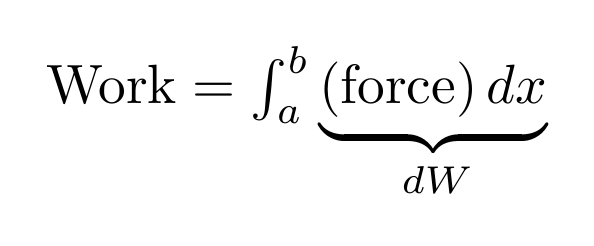
\begin{tikzpicture}[scale=2,every node/.style={transform shape}]
    \node at (0,0) {
      $\mathrm{Work} = \int_a^b \underbrace{\mathrm{(force)}\d x}_{\d W}$
    };
  \end{tikzpicture}
\end{image}
Let's try some examples:
\begin{example}
  How much work is performed pulling a $60\unit{m}$ climbing rope up a
  cliff face, where the rope has a mass of $66\unit{g}/\unit{m}$?
  \begin{explanation}
    Let $y$ be the distance we have pulled the rope.  The force $F(y)$
    on the rope is always ``large'' (read: not infinitesimal), but the
    force is changing as we pull the rope up.  If we think of pulling
    the rope up only an infinitesimal amount $\d y$, then the force
    will be constant over that infinitesimal distance, so the
    infinitesimal amount of work done by moving the rope through $\d
    y$ at height $y$ is
    \[
    \d W = F(y) \d y.
    \]
    Integrating these infinitesimal amounts of work from $y=0$ to
    $y=60$ should yield the total amount of work done.  In this
    example, the mass of the rope remaining after $y$ feet have been
    pulled up is
    \[
    \mathrm{mass}(y) = \answer[given]{(0.066)(60-y)} \unit{kg}.
    \]
    \begin{hint}
      There are $60-y$ feet of rope, at a density of $66\unit{g}/\unit{m}$, so
      the total mass of the rope is $(60-y)66\unit{g}$.  Converted to kilograms,
      this is $(60-y)(0.066)\unit{kg}$.
    \end{hint}
    The force due to gravity on the rope after $y$ feet have been pulled up is
    \[
    F(y) = \answer[given]{(0.066)(60-y)(9.8)} \unit{N} 
    \]
    \begin{hint}
      To get the force due to gravity from the mass, we just
      multiply the mass by standard gravity, $g = 9.8
      \frac{\unit{m}}{\unit{s}^2}$.  Since we have already written
      our mass in $\unit{kg}$, we obtain $F(y) = (0.066)(60-y)(9.8)
      \unit{N}$.
    \end{hint}
    The total work done is
    \[
    \int_0^{60} F(y) \d y = \answer[given]{1164.24} \unit{J}
    \]
    \begin{hint}
      \begin{align*}
	\int_0^{60} F(y) \d y &= \int_0^{60}(0.066)(60-y)(9.8) \d y \\
	&= (0.066)(9.8) \eval{\answer[given]{60y - \frac{y^2}{2}}}_0^{60}\\
	&=(0.066)(9.8)(1800)\\
	&= 1164.24
      \end{align*}
    \end{hint}    
    By comparison, consider the work done in lifting the entire rope
    $60$ meters. The rope weights
    \[
    60\times 0.066 \times 9.8 = 38.808\unit{N},
    \]
    so the work applying this force for $60$ meters is
    \[
    60\times 38.808 = 2328.48 \unit{J}.
    \]
    This is exactly twice the work calculated before, we leave it to
    the young mathematician to understand why.
  \end{explanation}
\end{example}

We can also do ``spring'' problems, for this we need \textit{Hooke's
  Law}:

\begin{definition}[Hooke's Law]\index{Hooke's Law}
  The force required to compress or stretch a spring $x$ units from
  its natural length (its unstretched length) is proportional to $x$.
  That is, this force is
  \[
  F(x) = k\cdot x
  \]
  for some constant $k$, known as the \dfn{spring constant}.
\end{definition}

\begin{warning}
  We expect you to memorize Hooke's law, and be able to use it in similar work problems.
\end{warning}

\begin{question}
  If a a force of $1\unit{N}$ stretches a given spring $2\unit{cm}$,
  then how far will a force of $5\unit{N}$ stretch the spring?
  \begin{prompt}
    The spring will stretch $\answer{10}\unit{cm}$.
  \end{prompt}
  \begin{question}
    What is the spring constant in this case?
    \begin{hint}
      Convert the distances to meters.
    \end{hint}
    \begin{prompt}
      $k= \answer{50}\unit{N}/\unit{m}$.
    \end{prompt}
  \end{question}
\end{question}
  
\begin{example}
  Say a force of $20\unit{lb}$ stretches a spring from its natural
  length of $7$ inches to a length of $12$ inches. How much work was
  performed in stretching the spring to this length?
  \begin{explanation}
    \begin{hint}
      This is a ``Large forces over infinitesimal distances'' problem.
    \end{hint}
    Let $x$ be the amount we have stretched the spring beyond its
    natural length in inches, and let $F(x)$ be the force exerted by
    the spring at this distance in pounds.  We have that $F(0)=0$,
    $F(5) = 20$, and we know that it is linear in the distance by
    Hooke's law.  So the ``large force'' involved is $F(x) = 4x$.  The
    work done by moving the spring from $x$ to $x+\d x$ (an
    infinitesimal distance) is
    \[
    \d W = \answer[given]{4x} \d x.
    \]
    We need to accumulate these ``large forces over infinitesimal
    distances'' from $x=0$ to $x=5$.
    \begin{align*}
      \mathrm{Work} &= \int_0^5 4x \d x\\
      &= \eval{\answer[given]{2x^2}}_0^5\\
      &=50
    \end{align*}
  \begin{hint}
    We need the answer to be in foot-pounds not inch-pounds, so we convert
    inches to feet to obtain $\frac{50}{12}$ foot-pounds.
  \end{hint}
    \[
    \mathrm{Work} = \answer[given]{\frac{50}{12}} \unit{ft}\cdot\unit{lb}.
    \]
  \end{explanation}
\end{example}







\subsection{Accumulating infinitesimal forces over large distances}

The basic set-up for these integrals is as follows:
  \begin{image}
  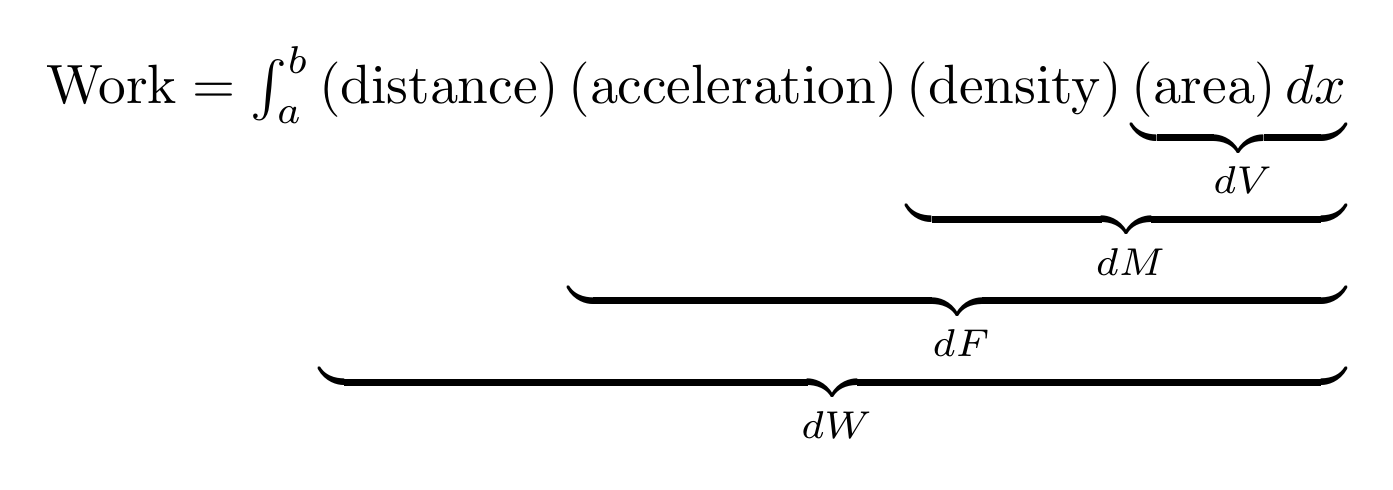
\begin{tikzpicture}[scale=2,every node/.style={transform shape}]
    \node at (0,0) {
      $\mathrm{Work} = \int_a^b \underbrace{
        \mathrm{(distance)}
        \underbrace{
          \mathrm{(acceleration)}
          \underbrace{
            \mathrm{(density)}
            \underbrace{
              \mathrm{(area)}\d x}_{\d V}}_{\d M}}_{\d F}}_{\d W}$
    };
  \end{tikzpicture}
  \end{image}
  Where $V$ represents volume, $M$ represents mass, $F$ represents
  force, and $W$ represents work as a function of $x$, position.
  Let's try some examples:
  
\begin{example}
  A cylindrical storage tank with a radius of $10 \unit{ft}$ and a
  height of $30\unit{ft}$ is filled with water, which weighs
  approximately $62.4 \unit{lb}/\unit{ft}^3$. Compute the amount of
  work performed by pumping the water up to a point $5$ feet above the
  top of the tank.
  \begin{explanation}
    If we were lifting the entire tank $35$ feet, there would be no
    need for calculus, and we could treat this as a simple
    multiplication problem.  Unfortunately, \textbf{different parts of
      the water are traveling different distances}; the water at the
    top of the tank has a much shorter distance to travel than the
    water at the bottom of the tank.
	
    Our approach will be to look at infinitesimal slabs of water.  All
    of the water in such a slab will have to travel the same distance
    to the top of the tank.  The force due to gravity on this slab
    will be infinitesimal because the volume of the water is
    infinitesimal.
    
    Let $y$ be the position of the slab as measured from the bottom of
    the cylindrical tank and $\d y$ be the thickness of the slab.

    \begin{image}
      \begin{tikzpicture}
        \draw[penColor,very thick] (0,2) ellipse (2 and .7);
        \draw[very thick,penColor!20!background] (2,-2) arc (0:180:2 and .7);% top half of ellipse
        \draw[very thick,penColor] (-2,-2) arc (180:360:2 and .7);% bottom half of ellipse
      
        \draw[very thick,penColor!20!background] (2,0) arc (0:180:2 and .7);% top half of ellipse
        \draw[very thick,penColor] (-2,0) arc (180:360:2 and .7);% bottom half of ellipse
        \draw[very thick,penColor!20!background] (2,0.1) arc (0:180:2 and .7);% top half of ellipse
        \draw[very thick,penColor] (-2,0.1) arc (180:360:2 and .7);% bottom half of ellipse
        
        \draw[decoration={brace,mirror, raise=.1cm},decorate,thin] (-2,0)--(-2,-2);
        
        \node [penColor] at (-2.4,-1) {$y$};
        \node [above,penColor] at (2.2,-0.3) {$\d y$};
        
        \draw[penColor, very thick] (2,2) -- (2,-2);
        \draw[penColor, very thick] (-2,2) -- (-2,-2);
      \end{tikzpicture}
    \end{image}
    Each slab has a volume of
    \[
    \pi r^2 \d y = \answer[given]{100}\pi\d y.
    \]
    Thus the weight of each slab is
    \[
    \answer[given]{62.4}(100\pi)\d y = \answer[given]{6240}\pi \d y.
    \]
    Note that this is already a force, not a mass measurement, so we
    do not have to convert it further.  Each slab has to move a
    distance of $\answer[given]{30-y +5}$, so the work done by moving
    each slab is
    \[
    \d W = 6240 \pi (\answer[given]{35-y}) \d y.
    \]
    Thus the total work done by pumping all of the water to the top is
    \begin{align*}
      \mathrm{Work} &= \int_0^{30} 6240 \pi (35-y) \d y\\
      &= 6240 \pi \eval{\answer[given]{35y-\frac{1}{2}y^2}}_0^{30}\\
      &=  3744000 \pi \unit{ft}\cdot\unit{lbs}.
    \end{align*}
  \end{explanation}
\end{example}


\end{document}
